\begin{figure}[!]
    \centering
    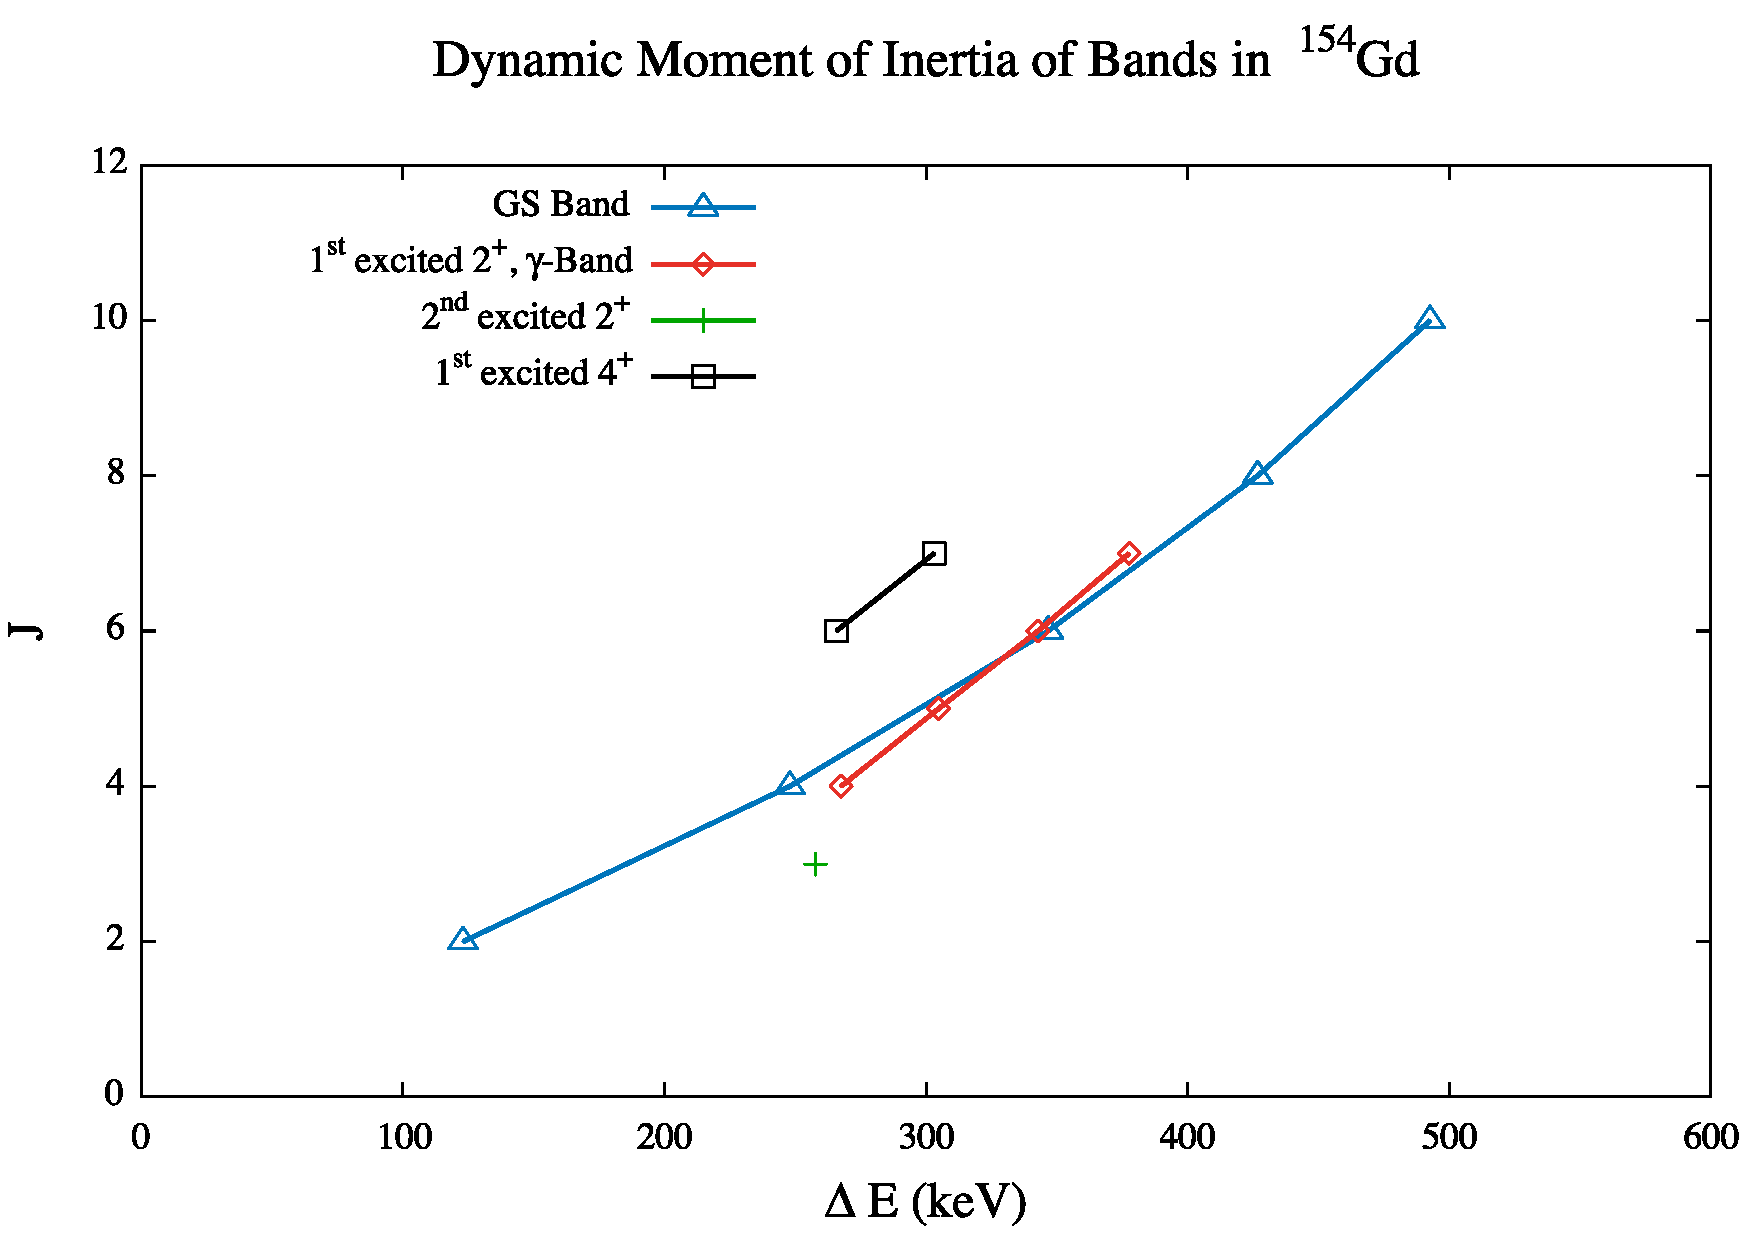
\includegraphics[scale=0.45]{Discussion/154_Dynamic.pdf}
    \caption{The dynamic moments of inertia of the ground state, $K=2^+_1$ and $K=4^+_1$ bands. As is seen visually and with the slopes, the ground state band and the $\gamma$ band have similar moments of inertia. However, they do not overlap within their standard deviations. The $K=2^+_1$ and $K=4^+_1$ bands have identical moments of inertia, indicating the $K=4^+_1$ band is an excitation built of the $K=2^+_1$ band.}
    \label{fig:154_Dynamic}
\end{figure}